% Created by tikzDevice version 0.12.4 on 2023-07-12 07:56:27
% !TEX encoding = UTF-8 Unicode
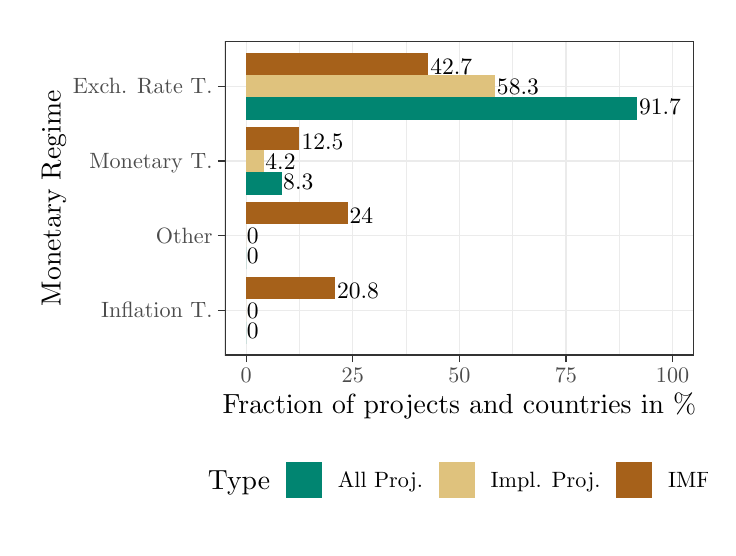
\begin{tikzpicture}[x=1pt,y=1pt]
\definecolor{fillColor}{RGB}{255,255,255}
\path[use as bounding box,fill=fillColor,fill opacity=0.00] (0,0) rectangle (245.72,180.67);
\begin{scope}
\path[clip] (  0.00,  0.00) rectangle (245.72,180.67);
\definecolor{drawColor}{RGB}{255,255,255}
\definecolor{fillColor}{RGB}{255,255,255}

\path[draw=drawColor,line width= 0.5pt,line join=round,line cap=round,fill=fillColor] ( -0.00,  0.00) rectangle (245.72,180.68);
\end{scope}
\begin{scope}
\path[clip] ( 71.26, 62.35) rectangle (240.72,175.67);
\definecolor{fillColor}{RGB}{255,255,255}

\path[fill=fillColor] ( 71.26, 62.35) rectangle (240.72,175.67);
\definecolor{drawColor}{gray}{0.92}

\path[draw=drawColor,line width= 0.3pt,line join=round] ( 98.22, 62.35) --
	( 98.22,175.67);

\path[draw=drawColor,line width= 0.3pt,line join=round] (136.73, 62.35) --
	(136.73,175.67);

\path[draw=drawColor,line width= 0.3pt,line join=round] (175.25, 62.35) --
	(175.25,175.67);

\path[draw=drawColor,line width= 0.3pt,line join=round] (213.76, 62.35) --
	(213.76,175.67);

\path[draw=drawColor,line width= 0.5pt,line join=round] ( 71.26, 78.54) --
	(240.72, 78.54);

\path[draw=drawColor,line width= 0.5pt,line join=round] ( 71.26,105.52) --
	(240.72,105.52);

\path[draw=drawColor,line width= 0.5pt,line join=round] ( 71.26,132.50) --
	(240.72,132.50);

\path[draw=drawColor,line width= 0.5pt,line join=round] ( 71.26,159.49) --
	(240.72,159.49);

\path[draw=drawColor,line width= 0.5pt,line join=round] ( 78.97, 62.35) --
	( 78.97,175.67);

\path[draw=drawColor,line width= 0.5pt,line join=round] (117.48, 62.35) --
	(117.48,175.67);

\path[draw=drawColor,line width= 0.5pt,line join=round] (155.99, 62.35) --
	(155.99,175.67);

\path[draw=drawColor,line width= 0.5pt,line join=round] (194.50, 62.35) --
	(194.50,175.67);

\path[draw=drawColor,line width= 0.5pt,line join=round] (233.02, 62.35) --
	(233.02,175.67);
\definecolor{fillColor}{RGB}{1,133,113}

\path[fill=fillColor] ( 78.97, 66.40) rectangle ( 78.97, 74.49);

\path[fill=fillColor] ( 78.97,120.36) rectangle ( 91.80,128.46);

\path[fill=fillColor] ( 78.97,147.34) rectangle (220.18,155.44);

\path[fill=fillColor] ( 78.97, 93.38) rectangle ( 78.97,101.47);
\definecolor{fillColor}{RGB}{223,194,125}

\path[fill=fillColor] ( 78.97, 74.49) rectangle ( 78.97, 82.59);

\path[fill=fillColor] ( 78.97,128.46) rectangle ( 85.38,136.55);

\path[fill=fillColor] ( 78.97,155.44) rectangle (168.83,163.53);

\path[fill=fillColor] ( 78.97,101.47) rectangle ( 78.97,109.57);
\definecolor{fillColor}{RGB}{166,97,26}

\path[fill=fillColor] ( 78.97, 82.59) rectangle (111.06, 90.68);

\path[fill=fillColor] ( 78.97,136.55) rectangle ( 98.22,144.65);

\path[fill=fillColor] ( 78.97,163.53) rectangle (144.76,171.63);

\path[fill=fillColor] ( 78.97,109.57) rectangle (115.87,117.66);
\definecolor{drawColor}{RGB}{0,0,0}

\node[text=drawColor,anchor=base west,inner sep=0pt, outer sep=0pt, scale=  0.85] at ( 79.18, 68.40) {0};

\node[text=drawColor,anchor=base west,inner sep=0pt, outer sep=0pt, scale=  0.85] at ( 92.35,122.37) {8.3};

\node[text=drawColor,anchor=base west,inner sep=0pt, outer sep=0pt, scale=  0.85] at (220.94,149.35) {91.7};

\node[text=drawColor,anchor=base west,inner sep=0pt, outer sep=0pt, scale=  0.85] at ( 79.18, 95.39) {0};

\node[text=drawColor,anchor=base west,inner sep=0pt, outer sep=0pt, scale=  0.85] at ( 79.18, 75.60) {0};

\node[text=drawColor,anchor=base west,inner sep=0pt, outer sep=0pt, scale=  0.85] at ( 85.93,129.56) {4.2};

\node[text=drawColor,anchor=base west,inner sep=0pt, outer sep=0pt, scale=  0.85] at (169.59,156.55) {58.3};

\node[text=drawColor,anchor=base west,inner sep=0pt, outer sep=0pt, scale=  0.85] at ( 79.18,102.58) {0};

\node[text=drawColor,anchor=base west,inner sep=0pt, outer sep=0pt, scale=  0.85] at (111.82, 82.80) {20.8};

\node[text=drawColor,anchor=base west,inner sep=0pt, outer sep=0pt, scale=  0.85] at ( 98.98,136.76) {12.5};

\node[text=drawColor,anchor=base west,inner sep=0pt, outer sep=0pt, scale=  0.85] at (145.52,163.74) {42.7};

\node[text=drawColor,anchor=base west,inner sep=0pt, outer sep=0pt, scale=  0.85] at (116.30,109.78) {24};
\definecolor{drawColor}{gray}{0.20}

\path[draw=drawColor,line width= 0.5pt,line join=round,line cap=round] ( 71.26, 62.35) rectangle (240.72,175.67);
\end{scope}
\begin{scope}
\path[clip] (  0.00,  0.00) rectangle (245.72,180.67);
\definecolor{drawColor}{gray}{0.30}

\node[text=drawColor,anchor=base east,inner sep=0pt, outer sep=0pt, scale=  0.80] at ( 66.76, 75.78) {Inflation T.};

\node[text=drawColor,anchor=base east,inner sep=0pt, outer sep=0pt, scale=  0.80] at ( 66.76,102.77) {Other};

\node[text=drawColor,anchor=base east,inner sep=0pt, outer sep=0pt, scale=  0.80] at ( 66.76,129.75) {Monetary T.};

\node[text=drawColor,anchor=base east,inner sep=0pt, outer sep=0pt, scale=  0.80] at ( 66.76,156.73) {Exch. Rate T.};
\end{scope}
\begin{scope}
\path[clip] (  0.00,  0.00) rectangle (245.72,180.67);
\definecolor{drawColor}{gray}{0.20}

\path[draw=drawColor,line width= 0.5pt,line join=round] ( 68.76, 78.54) --
	( 71.26, 78.54);

\path[draw=drawColor,line width= 0.5pt,line join=round] ( 68.76,105.52) --
	( 71.26,105.52);

\path[draw=drawColor,line width= 0.5pt,line join=round] ( 68.76,132.50) --
	( 71.26,132.50);

\path[draw=drawColor,line width= 0.5pt,line join=round] ( 68.76,159.49) --
	( 71.26,159.49);
\end{scope}
\begin{scope}
\path[clip] (  0.00,  0.00) rectangle (245.72,180.67);
\definecolor{drawColor}{gray}{0.20}

\path[draw=drawColor,line width= 0.5pt,line join=round] ( 78.97, 59.85) --
	( 78.97, 62.35);

\path[draw=drawColor,line width= 0.5pt,line join=round] (117.48, 59.85) --
	(117.48, 62.35);

\path[draw=drawColor,line width= 0.5pt,line join=round] (155.99, 59.85) --
	(155.99, 62.35);

\path[draw=drawColor,line width= 0.5pt,line join=round] (194.50, 59.85) --
	(194.50, 62.35);

\path[draw=drawColor,line width= 0.5pt,line join=round] (233.02, 59.85) --
	(233.02, 62.35);
\end{scope}
\begin{scope}
\path[clip] (  0.00,  0.00) rectangle (245.72,180.67);
\definecolor{drawColor}{gray}{0.30}

\node[text=drawColor,anchor=base,inner sep=0pt, outer sep=0pt, scale=  0.80] at ( 78.97, 52.34) {0};

\node[text=drawColor,anchor=base,inner sep=0pt, outer sep=0pt, scale=  0.80] at (117.48, 52.34) {25};

\node[text=drawColor,anchor=base,inner sep=0pt, outer sep=0pt, scale=  0.80] at (155.99, 52.34) {50};

\node[text=drawColor,anchor=base,inner sep=0pt, outer sep=0pt, scale=  0.80] at (194.50, 52.34) {75};

\node[text=drawColor,anchor=base,inner sep=0pt, outer sep=0pt, scale=  0.80] at (233.02, 52.34) {100};
\end{scope}
\begin{scope}
\path[clip] (  0.00,  0.00) rectangle (245.72,180.67);
\definecolor{drawColor}{RGB}{0,0,0}

\node[text=drawColor,anchor=base,inner sep=0pt, outer sep=0pt, scale=  1.00] at (155.99, 41.40) {Fraction of projects and countries in \%};
\end{scope}
\begin{scope}
\path[clip] (  0.00,  0.00) rectangle (245.72,180.67);
\definecolor{drawColor}{RGB}{0,0,0}

\node[text=drawColor,rotate= 90.00,anchor=base,inner sep=0pt, outer sep=0pt, scale=  1.00] at ( 11.89,119.01) {Monetary Regime};
\end{scope}
\begin{scope}
\path[clip] (  0.00,  0.00) rectangle (245.72,180.67);
\definecolor{fillColor}{RGB}{255,255,255}

\path[fill=fillColor] ( 60.11,  5.00) rectangle (251.88, 29.45);
\end{scope}
\begin{scope}
\path[clip] (  0.00,  0.00) rectangle (245.72,180.67);
\definecolor{drawColor}{RGB}{0,0,0}

\node[text=drawColor,anchor=base west,inner sep=0pt, outer sep=0pt, scale=  1.00] at ( 65.11, 13.78) {Type};
\end{scope}
\begin{scope}
\path[clip] (  0.00,  0.00) rectangle (245.72,180.67);
\definecolor{fillColor}{RGB}{255,255,255}

\path[fill=fillColor] ( 92.60, 10.00) rectangle (107.05, 24.45);
\end{scope}
\begin{scope}
\path[clip] (  0.00,  0.00) rectangle (245.72,180.67);
\definecolor{fillColor}{RGB}{1,133,113}

\path[fill=fillColor] ( 93.31, 10.71) rectangle (106.34, 23.74);
\end{scope}
\begin{scope}
\path[clip] (  0.00,  0.00) rectangle (245.72,180.67);
\definecolor{fillColor}{RGB}{255,255,255}

\path[fill=fillColor] (147.85, 10.00) rectangle (162.30, 24.45);
\end{scope}
\begin{scope}
\path[clip] (  0.00,  0.00) rectangle (245.72,180.67);
\definecolor{fillColor}{RGB}{223,194,125}

\path[fill=fillColor] (148.56, 10.71) rectangle (161.59, 23.74);
\end{scope}
\begin{scope}
\path[clip] (  0.00,  0.00) rectangle (245.72,180.67);
\definecolor{fillColor}{RGB}{255,255,255}

\path[fill=fillColor] (211.98, 10.00) rectangle (226.43, 24.45);
\end{scope}
\begin{scope}
\path[clip] (  0.00,  0.00) rectangle (245.72,180.67);
\definecolor{fillColor}{RGB}{166,97,26}

\path[fill=fillColor] (212.69, 10.71) rectangle (225.72, 23.74);
\end{scope}
\begin{scope}
\path[clip] (  0.00,  0.00) rectangle (245.72,180.67);
\definecolor{drawColor}{RGB}{0,0,0}

\node[text=drawColor,anchor=base west,inner sep=0pt, outer sep=0pt, scale=  0.80] at (112.05, 14.47) {All Proj.};
\end{scope}
\begin{scope}
\path[clip] (  0.00,  0.00) rectangle (245.72,180.67);
\definecolor{drawColor}{RGB}{0,0,0}

\node[text=drawColor,anchor=base west,inner sep=0pt, outer sep=0pt, scale=  0.80] at (167.30, 14.47) {Impl. Proj.};
\end{scope}
\begin{scope}
\path[clip] (  0.00,  0.00) rectangle (245.72,180.67);
\definecolor{drawColor}{RGB}{0,0,0}

\node[text=drawColor,anchor=base west,inner sep=0pt, outer sep=0pt, scale=  0.80] at (231.43, 14.47) {IMF};
\end{scope}
\end{tikzpicture}
